\subsubsection{Arquitectura Modular del Sistema}

El sistema de inteligencia artificial implementado se estructura en cuatro módulos funcionales especializados que operan de manera coordinada para lograr la autonomía del robot cosechador. Esta arquitectura modular permite la separación de responsabilidades, facilita el mantenimiento y posibilita la evolución independiente de cada componente.

El primer módulo, denominado \textbf{Sistema de Posicionamiento Visual}, tiene como función detectar desviaciones respecto a la posición ideal mediante el análisis de marcadores visuales de referencia. Este módulo calcula correcciones en tiempo real que compensan las holguras mecánicas acumulativas del sistema de movimiento, garantizando precisión submilimétrica en el alineamiento frente a cada estación de cultivo.

El segundo módulo corresponde al \textbf{Sistema de Clasificación de Cultivos}, responsable de determinar la presencia o ausencia de lechuga en cada estación mediante análisis morfológico de características extraídas de imágenes. La clasificación se basa en umbrales estadísticos derivados de un análisis exhaustivo de muestras representativas del entorno operativo.

El tercer módulo, \textbf{Sistema de Mapeo Autónomo}, construye una representación espacial completa del entorno de cultivo mediante exploración sistemática. Este módulo registra la posición y estado de cada estación, generando una base de datos espacial que sirve como entrada para la planificación de operaciones de cosecha.

Finalmente, el cuarto módulo de \textbf{Optimización de Trayectorias} procesa la información del mapa construido para generar rutas que minimizan el tiempo total de operación. Este módulo adapta el problema clásico del viajante a las restricciones geométricas y cinemáticas específicas del robot cartesiano.

\begin{figure}[h]
\centering
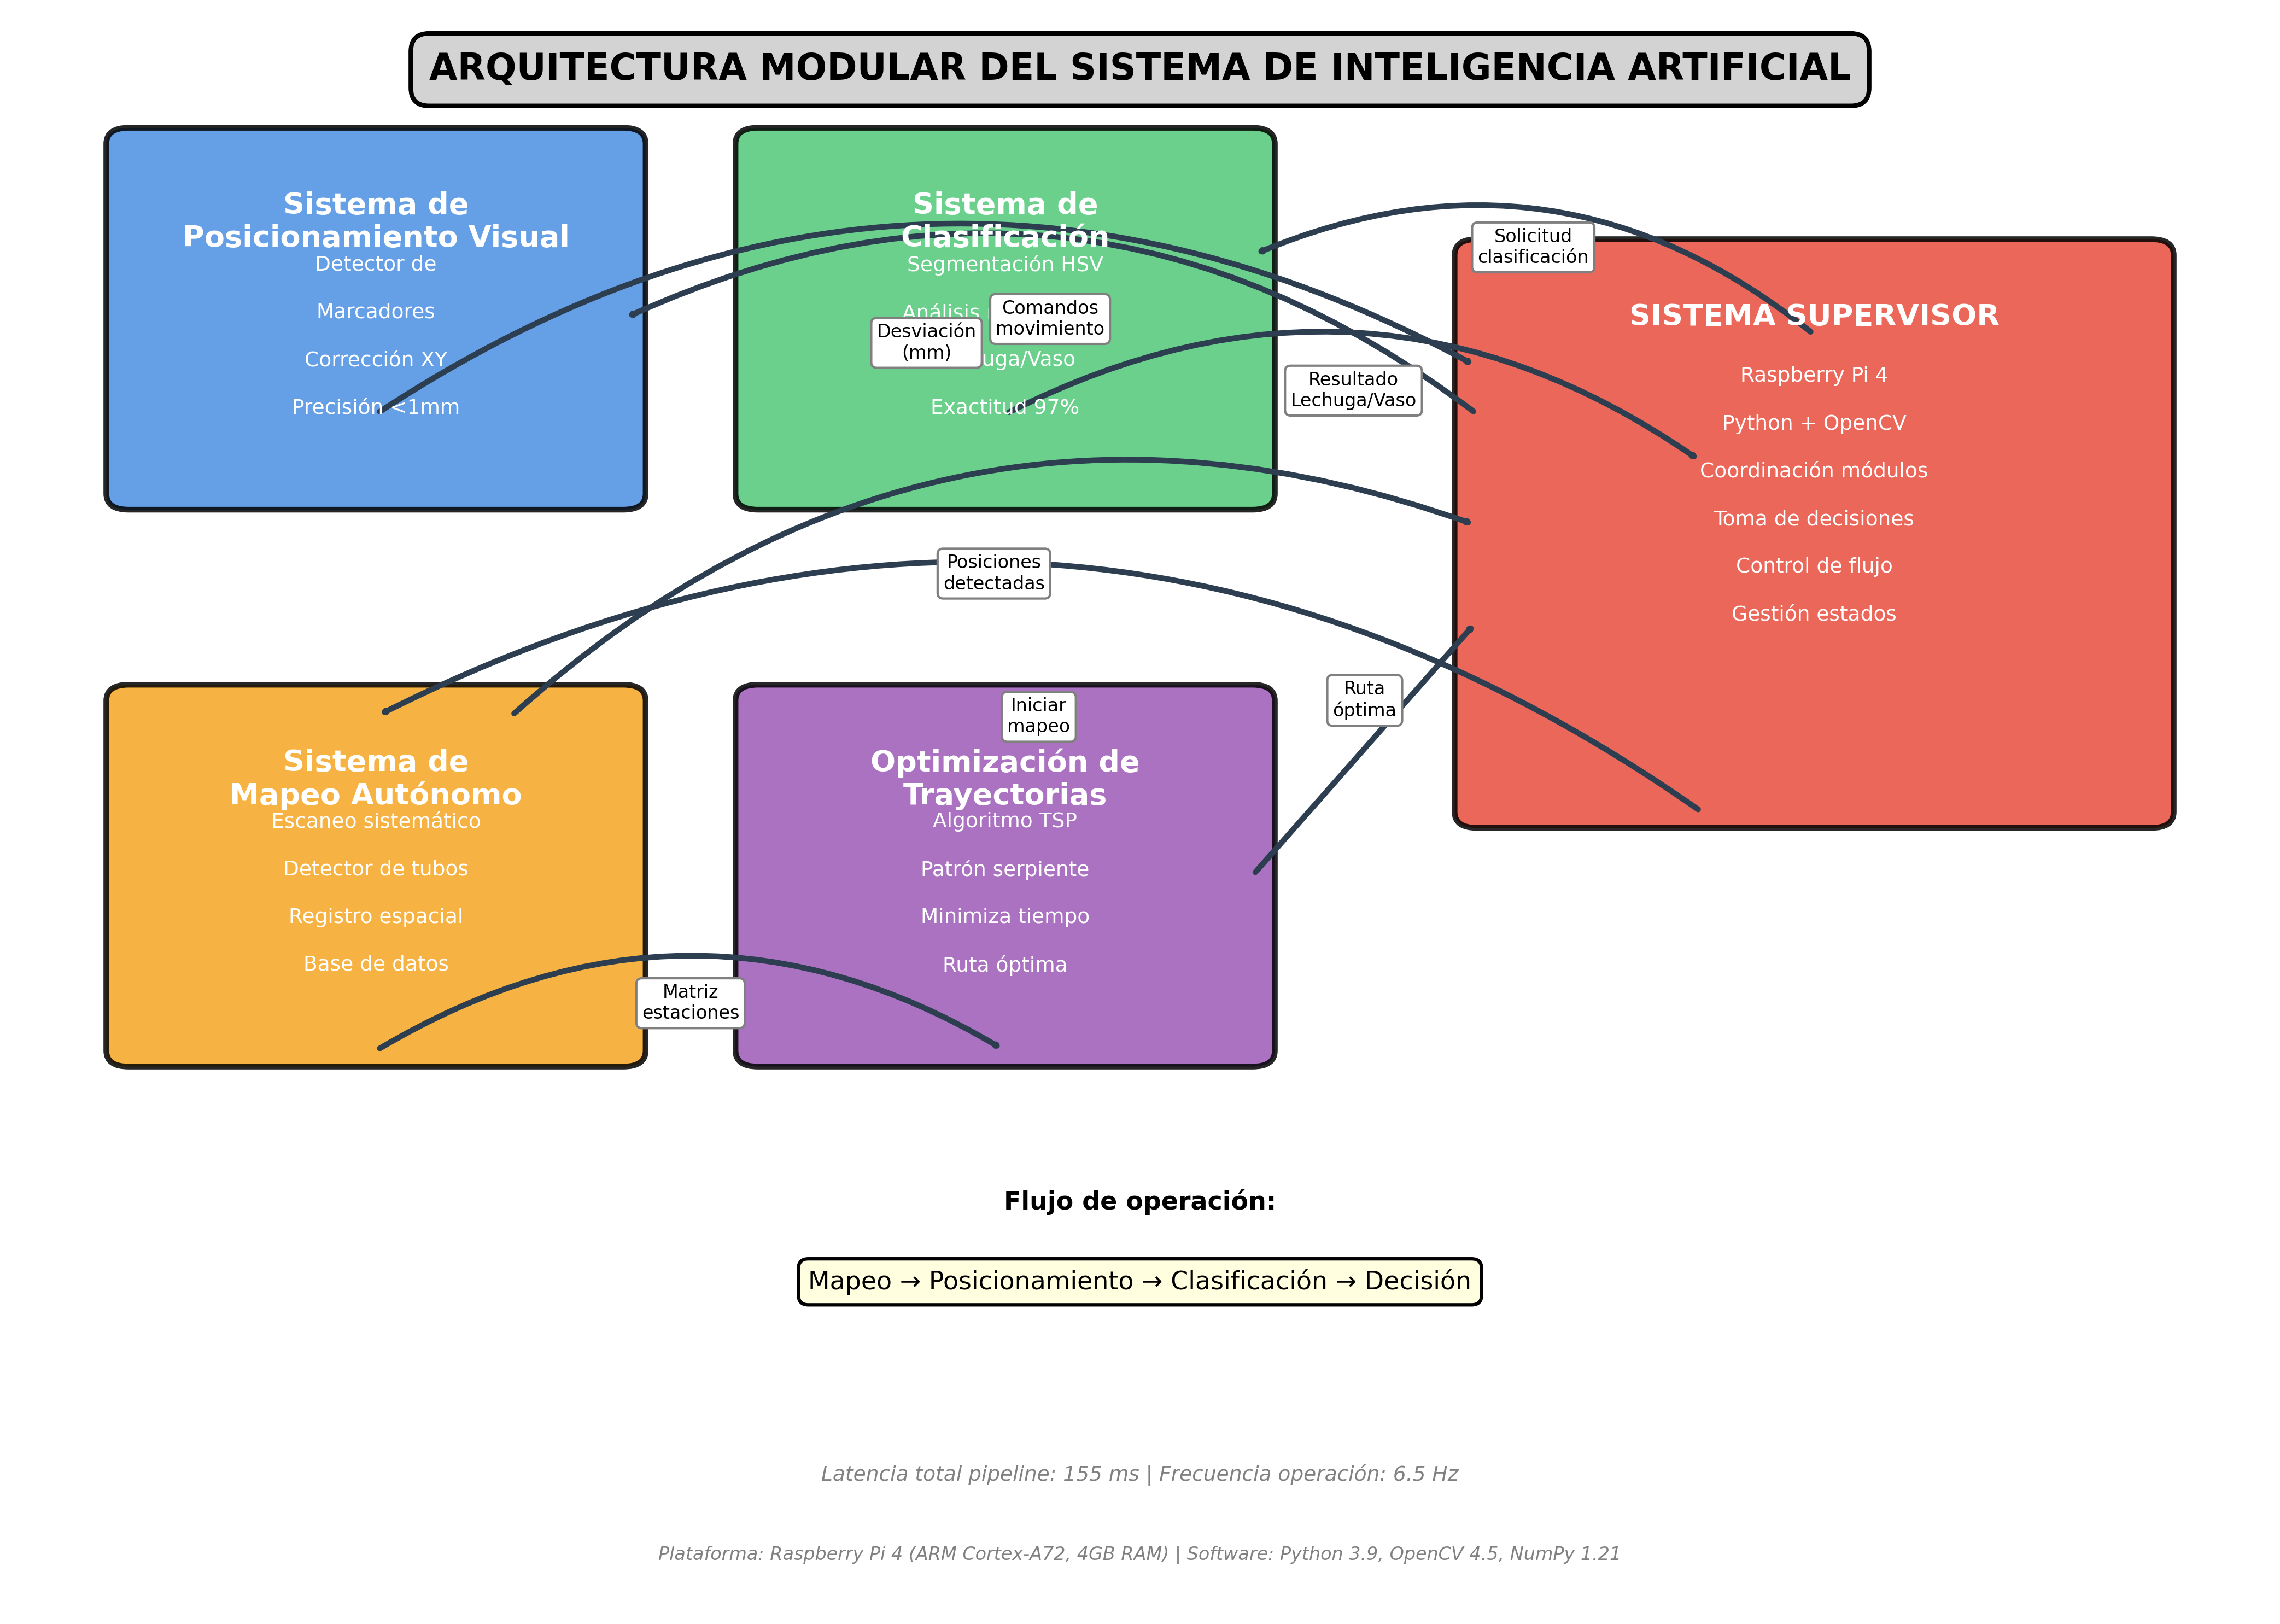
\includegraphics[width=0.85\textwidth]{imagenes/arquitectura_modular_ia.png}
\caption{Arquitectura modular del sistema de inteligencia artificial mostrando la interconexión entre los cuatro módulos principales y el flujo de información}
\label{fig:arquitectura_modular}
\end{figure}

\textbf{Flujo de Información entre Módulos}

La información fluye siguiendo una jerarquía de control bien definida. El módulo de mapeo identifica las estaciones objetivo que requieren atención. Para cada estación identificada, el módulo de posicionamiento ejecuta las correcciones visuales necesarias para garantizar el alineamiento preciso. Una vez posicionado correctamente, el módulo de clasificación determina el estado del cultivo. Finalmente, basándose en esta información, el sistema supervisor toma la decisión de ejecutar la cosecha o avanzar a la siguiente estación. Este flujo puede expresarse mediante la secuencia:

\begin{equation}
\text{Mapeo} \rightarrow \text{Posicionamiento} \rightarrow \text{Clasificación} \rightarrow \text{Decisión}
\end{equation}

Cada módulo expone interfaces funcionales bien definidas que permiten la invocación de operaciones específicas y el intercambio de datos estructurados. El módulo de posicionamiento recibe como entrada la imagen capturada y el eje a corregir, retornando la desviación calculada en milímetros. El módulo de clasificación procesa una imagen y retorna un valor booleano indicando presencia o ausencia de lechuga junto con un índice de confianza. El módulo de mapeo ejecuta la exploración completa y retorna una matriz que contiene coordenadas y estados de todas las estaciones. El módulo de trayectorias recibe esta matriz como entrada y genera una lista ordenada de coordenadas que define la secuencia óptima de visita.

\textbf{Selección de Plataforma Computacional}

La implementación del sistema de inteligencia artificial se realizó sobre una Raspberry Pi 4 Model B equipada con procesador ARM Cortex-A72 de cuatro núcleos operando a 1.5 GHz y 4 GB de memoria RAM tipo LPDDR4. Esta plataforma fue seleccionada por su capacidad de ejecutar algoritmos de visión por computadora en tiempo real manteniendo un consumo energético reducido, compatible con las restricciones del sistema embarcado del robot.

Las bibliotecas de software empleadas incluyen OpenCV versión 4.5 para procesamiento de imágenes y detección de contornos, NumPy versión 1.21 para operaciones matriciales de alto rendimiento necesarias en la calibración espacial, y PySerial para la comunicación mediante protocolo UART con el nivel regulatorio. La elección de Python como lenguaje de implementación se fundamenta en su amplio ecosistema de bibliotecas científicas, la velocidad de desarrollo y prototipado, y un rendimiento suficiente para las frecuencias de operación requeridas por el sistema.

El sistema operativo Raspberry Pi OS, basado en Debian, proporciona soporte nativo para los controladores de cámara mediante la interfaz Video4Linux2, permitiendo la captura de imágenes sin configuración adicional. La arquitectura ARM del procesador incluye extensiones SIMD que aceleran las operaciones vectoriales intensivas empleadas en el procesamiento de imágenes.

\subsubsection{Pipeline General de Procesamiento}

El procesamiento de imágenes sigue un pipeline estructurado en siete etapas secuenciales que transforman las imágenes crudas capturadas en información accionable para el control del robot. Cada etapa aplica transformaciones específicas que progresivamente refinan la información hasta extraer las características relevantes para la toma de decisiones.

La primera etapa corresponde a la \textbf{adquisición de imágenes} RGB con resolución de 1920×1080 píxeles mediante la cámara USB. Esta etapa presenta una latencia aproximada de 50 milisegundos que incluye el tiempo de exposición del sensor, la lectura de los datos del array de píxeles y la transferencia mediante interfaz USB 2.0 hacia la memoria del sistema.

La segunda etapa realiza el \textbf{preprocesamiento} mediante la conversión del espacio de color RGB al espacio HSV. Esta transformación, fundamentada en la teoría presentada en el marco teórico (Sección 2.2.1), separa la información cromática (matiz y saturación) de la información de luminosidad (valor), proporcionando robustez ante variaciones de iluminación ambiental. La conversión se ejecuta aplicando las ecuaciones de transformación estándar RGB-HSV sobre cada píxel de la imagen. El tiempo de procesamiento de esta operación es de aproximadamente 15 milisegundos, aprovechando las optimizaciones vectoriales de la biblioteca OpenCV.

La tercera etapa corresponde a la \textbf{segmentación}, donde se aplican operaciones de umbralización específicas según el módulo activo. Para el módulo de posicionamiento se extrae el canal V y se aplica umbralización inversa con valor de referencia de 50, destacando las regiones oscuras correspondientes a las cintas de referencia. Para el módulo de clasificación se emplea segmentación por rango cromático en los tres canales HSV, definiendo límites inferior y superior que aíslan las tonalidades verdes correspondientes a vegetación. Esta etapa requiere 20 milisegundos de procesamiento.

La cuarta etapa implementa \textbf{refinamiento morfológico} mediante operaciones de cierre y apertura, aplicando los fundamentos teóricos descritos en la Sección 2.2.1 del marco teórico. La operación de cierre elimina pequeños huecos dentro de las regiones de interés, mientras que la apertura elimina píxeles aislados correspondientes a ruido. Ambas operaciones emplean un elemento estructurante rectangular de 3×3 píxeles. El costo computacional total de estas operaciones morfológicas es de 25 milisegundos.

La quinta etapa ejecuta la \textbf{detección de contornos} mediante el algoritmo de Suzuki-Abe, identificando las fronteras de las regiones segmentadas. Este algoritmo, cuya fundamentación matemática se presentó en la Sección 2.2.2, construye una representación jerárquica de los contornos detectados. Se emplea el modo de extracción de contornos externos únicamente, ya que las estructuras de interés no presentan huecos internos relevantes. La aproximación de contornos se realiza mediante compresión de puntos colineales, reduciendo el uso de memoria. Esta operación requiere aproximadamente 30 milisegundos de procesamiento.

La sexta etapa calcula \textbf{descriptores geométricos} de los contornos detectados. Se calculan el área mediante conteo de píxeles interiores, el centroide mediante momentos de imagen de orden cero y uno, el perímetro mediante suma de distancias euclidianas entre puntos consecutivos, y el rectángulo delimitador que encierra completamente al contorno. Estos descriptores constituyen las características cuantitativas empleadas para la toma de decisiones en los módulos de posicionamiento y clasificación. El tiempo de cálculo es de aproximadamente 10 milisegundos.

Finalmente, la séptima etapa genera el \textbf{comando de acción} correspondiente basándose en las características extraídas. Para el módulo de posicionamiento, esto corresponde al cálculo de la desviación en píxeles respecto al centro de la imagen y su posterior conversión a milímetros mediante los coeficientes de calibración. Para el módulo de clasificación, corresponde a la evaluación del área del contorno principal contra el umbral estadístico establecido, resultando en una decisión binaria de presencia o ausencia de lechuga. Esta etapa final requiere menos de 5 milisegundos.

El tiempo total de procesamiento del pipeline completo se obtiene mediante la suma de las latencias individuales:

\begin{equation}
T_{total} = T_{adq} + T_{prep} + T_{seg} + T_{morf} + T_{cont} + T_{desc} + T_{dec}
\end{equation}

\begin{equation}
T_{total} = 50 + 15 + 20 + 25 + 30 + 10 + 5 = 155 \text{ ms}
\end{equation}

Esta latencia total permite una frecuencia de operación de:

\begin{equation}
f = \frac{1}{T_{total}} = \frac{1}{0.155} \approx 6.5 \text{ Hz}
\end{equation}

Esta frecuencia es suficiente para el control en tiempo real considerando que las velocidades de movimiento del robot se encuentran en el rango de 5 a 10 cm/s, lo que implica desplazamientos de 7.75 a 15.5 mm entre capturas consecutivas.

\begin{figure}[h]
\centering
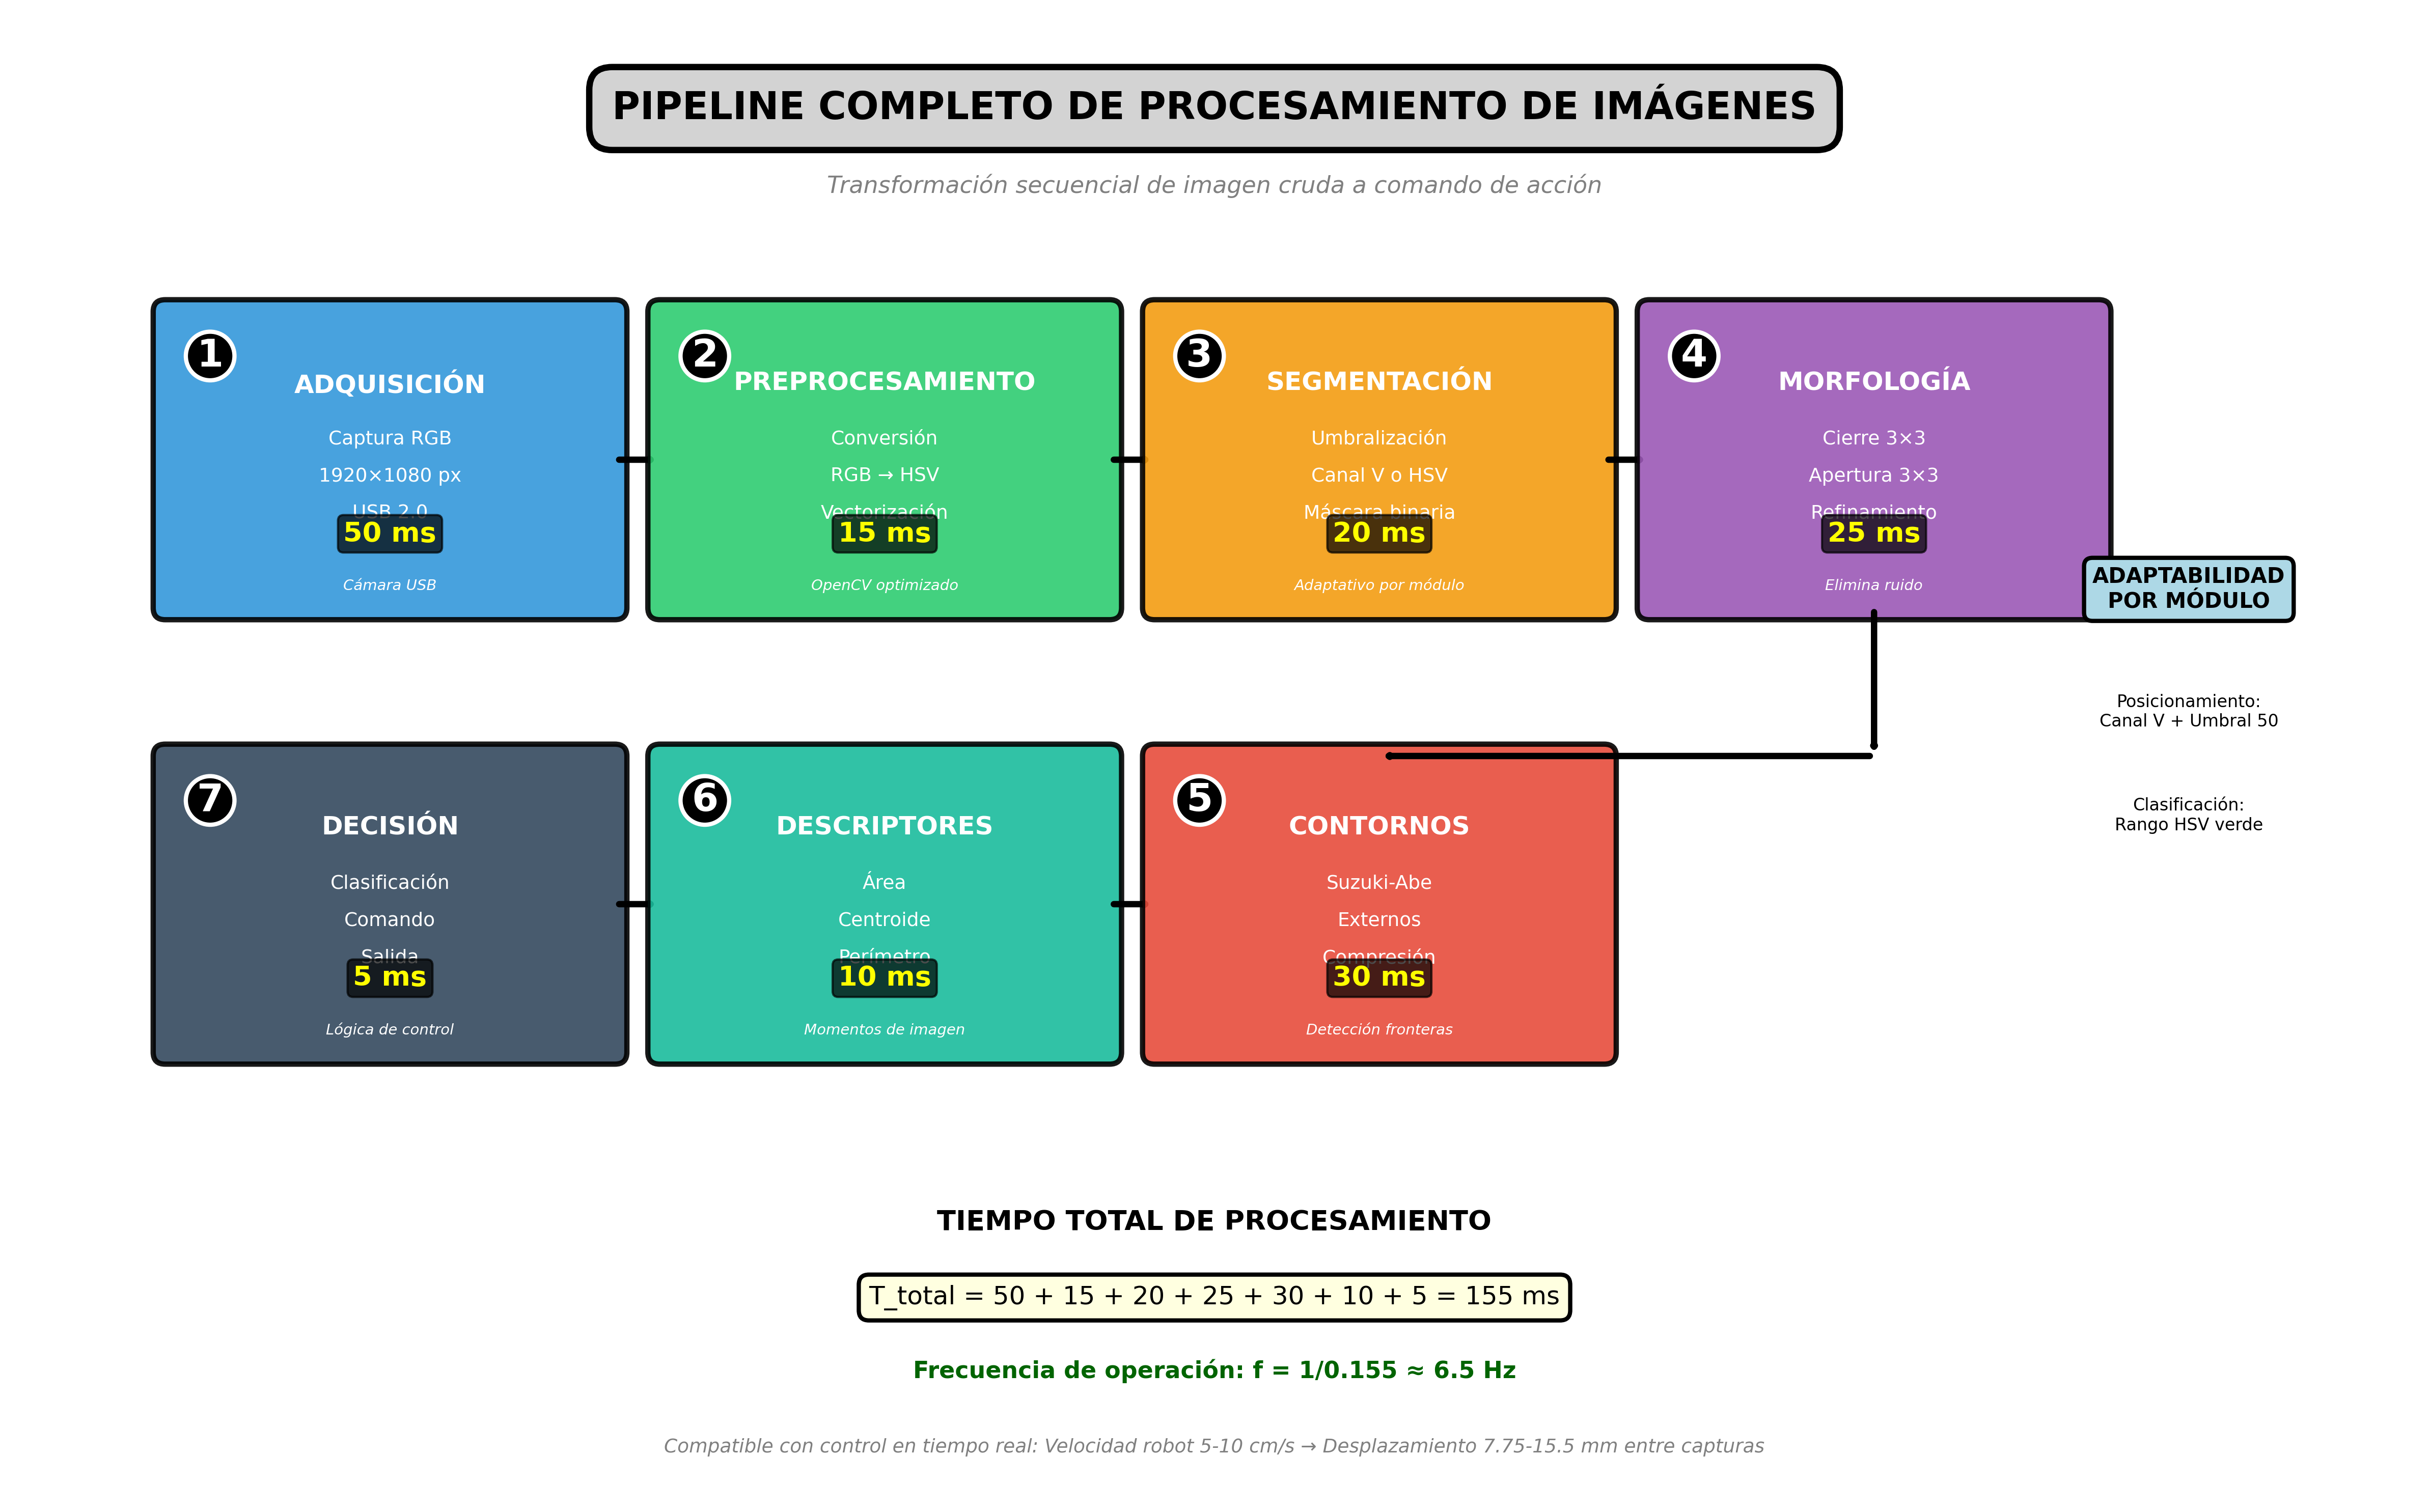
\includegraphics[width=0.95\textwidth]{imagenes/pipeline_procesamiento_completo.png}
\caption{Pipeline completo de procesamiento de imágenes mostrando las siete etapas secuenciales con sus tiempos característicos de ejecución}
\label{fig:pipeline_completo}
\end{figure}

El pipeline implementa un diseño adaptable que modifica su configuración según el módulo activo. Para el módulo de posicionamiento se utiliza únicamente el canal V del espacio HSV con umbralización inversa, enfocándose en la detección de elementos de alto contraste. Para el módulo de clasificación se emplean los tres canales HSV con segmentación por rango cromático, permitiendo la discriminación de vegetación verde. Esta adaptabilidad permite optimizar el procesamiento según los requerimientos específicos de cada tarea, manteniendo la latencia dentro de límites aceptables para el control en tiempo real.